\documentclass[12pt,a4paper]{report}
\usepackage[utf8]{inputenc}
\usepackage{amsmath}
\usepackage{amsfonts}
\usepackage{amssymb}
\usepackage{graphicx}
\usepackage{pgfplots}      % For plotting graphs
\usepackage{booktabs}
\usepackage{algorithm}
\usepackage{algpseudocode}
\usepackage{subcaption}
\usepackage[english]{babel}
\usepackage[export]{adjustbox}
\usepackage{enumerate}
\usepackage[left=3.5cm,right=2.5cm,top=2.5cm,bottom=2.5cm]{geometry}
\usepackage{lineno}
\usepackage{cite}
\usepackage{acronym}
\usepackage{multicol}      % For arranging items horizontally
\renewcommand{\baselinestretch}{1.5}

\begin{document}

	\begin{center}
    \scalebox{3}{\textbf{SAMPLING}}  % 3 scales the text size

		\vspace*{30pt}
		
		\textbf{\\
			\it{Assignment for Internal Marks}\\}
		\vspace{20pt}
		\textbf{Bachelor of Technology\\}
		in\\
		\vspace{3pt}
		{ELECTRICAL ENGINEERING}\\
		\vspace{40pt}
		
		\textbf{
			VANSH KUMAR GAUTAM(23BEE116)\\
                VANSHIKA(23BEE117)\\
                VINAYAK TIWARI(23BEE118)\\
                VEDANSH TYAGI(23BEE119)\\
                YASH SISODIA(23BEE120)\\
                YASHITA GUPTA(23BEE121)\\
                YASHVANT SINGH (23BEE122)\\
                YOGESH SHARMA(23BEE123)\\
                YUVRAJ SHARMA(23BEE124)\\
                PRATYUSH DIXIT(23BEE125)\\
            }\\
            
		\vspace{30pt}
		\includegraphics[width=0.3\textwidth]{./n-i-t-hamirpur-logo-k9i9rshtvwz2dvm5.png} \\
		\vspace{30pt}
		\textit{Under the kind guidance of}\\
		\textbf{DR. PANKAJ KUMAR MISHRA}\\
		\textit
		
		
		\vspace{20pt}
		
	\end{center}
\pagenumbering{gobble}

\newpage % Start the next page for additional content

\section*{Problems with Continuous Signals}

Continuous-time signals, though often representing physical phenomena accurately, present several challenges, particularly in processing, transmission, and storage. Here are the main problems associated with continuous-time (analog) signals:

\begin{itemize}
    \item \textbf{Susceptibility to Noise and Interference}\\
    Continuous signals are highly vulnerable to noise, distortion, and interference, especially during transmission. Small distortions or environmental interference can alter the signal and degrade the quality of the information.
    
    \item \textbf{Difficulty in Storage and Processing}\\
    Storing and processing continuous signals requires significant resources. Analog storage systems, such as tapes or magnetic disks, have limitations in terms of storage capacity, longevity, and degradation over time. Processing analog signals also requires complex analog circuits that lack the flexibility and accuracy of digital processing.
    
    \item \textbf{Complex Hardware Requirements}\\
    Manipulating continuous signals requires dedicated analog circuits, which are often complex, bulky, and sensitive to environmental changes. Analog components can degrade over time, causing issues like drift and calibration errors. Precise filtering, modulation, and amplification of analog signals often involve expensive hardware and limited precision, making digital alternatives preferable for many applications.
    
    \item \textbf{Bandwidth and Power Limitations}\\
    Transmitting analog signals can require significant bandwidth, as they cannot be efficiently compressed like digital signals. Additionally, transmission over long distances without signal degradation requires high power, which is inefficient and costly. Analog signals must often be amplified for long-distance transmission, which can introduce additional noise and degrade the signal further.
    
    \item \textbf{Loss of Data Integrity and Accuracy Over Time}\\
    Analog storage media degrade, causing the quality of stored analog signals to decrease. Audio and video recordings on analog tapes, for example, lose quality over time due to wear and environmental factors. Repeated duplication of analog signals also results in generational loss, with each copy introducing more distortion and loss of fidelity, unlike digital signals which can be copied without degradation.
\end{itemize}

In summary, while continuous signals represent information in its natural form, they are less practical for many modern applications due to their sensitivity to noise, storage inefficiencies, processing limitations, and higher maintenance needs. This is why many systems use sampling to convert analog signals to digital form for easier handling.

\section*{Why We Sample Signals}

We sample signals primarily to convert continuous-time (analog) signals into discrete-time (digital) signals, which enables processing, storage, and transmission in digital systems. Here are the main reasons why we sample signals:

\begin{itemize}
    \item \textbf{Digital Processing Compatibility}\\
    Most modern signal processing tools (computers, digital filters, etc.) work with digital signals. Sampling allows us to digitize analog signals so that they can be manipulated, analyzed, and processed using digital hardware and software.
    
    \item \textbf{Efficient Storage and Transmission}\\
    Analog signals require a large amount of storage and bandwidth. By sampling, we convert them into a digital format that can be compressed, transmitted, and stored more efficiently without requiring continuous-time reproduction.
    
    \item \textbf{Noise Reduction and Signal Integrity}\\
    Digital signals are less susceptible to degradation and noise compared to analog signals. Sampling enables digital representation, which can be transmitted and stored with greater resilience to noise, and errors can be corrected in digital systems.
    
    \item \textbf{Enabling Complex Signal Processing Techniques}\\
    Techniques like filtering, modulation, encryption, and compression are simpler to implement in digital form. Digital processing allows for flexible and precise control, automation, and adaptation that are difficult to achieve in the analog domain.
\end{itemize}





    % Title and author details here as before

    \newpage

    % Begin new content from the additional section
    \section*{\underline{\textbf{Sampling Theory}}}

    Sampling theory is essential in signal processing and telecommunications, as it allows for the transformation of continuous-time signals (analog) into discrete-time signals (digital). This process makes it possible to store, analyze, and manipulate signals on digital devices. The core principle behind sampling is the \textbf{Sampling Theorem} or \textbf{Nyquist-Shannon Theorem}. This theorem states that, to reconstruct a continuous signal accurately, the sampling rate must be at least twice the maximum frequency present in the signal. This minimum rate is called the Nyquist rate.

    \section*{\underline{\textbf{Sampling}}}

    Sampling is the reduction of a continuous-time signal to a discrete-time signal by capturing values of the signal at fixed intervals. This process is central to digital signal processing, as it bridges the gap between continuous and digital domains. When the sampling rate is sufficient, the original continuous signal can be reconstructed without information loss.

    \subsection*{\textbf{Steps in Sampling}}
    \begin{enumerate}
        \item \textbf{Continuous Signal:} The original analog signal is a continuous wave that varies smoothly over time.
        \item \textbf{Sampler:} The sampler device takes periodic snapshots of the continuous signal at a specific sampling rate.
        \item \textbf{Discrete Signal:} The sampled points form a discrete signal, which represents the original signal in digital form.
    \end{enumerate}

    \begin{center}
        \begin{multicols}{1}
            % Original Continuous Signal Diagram
            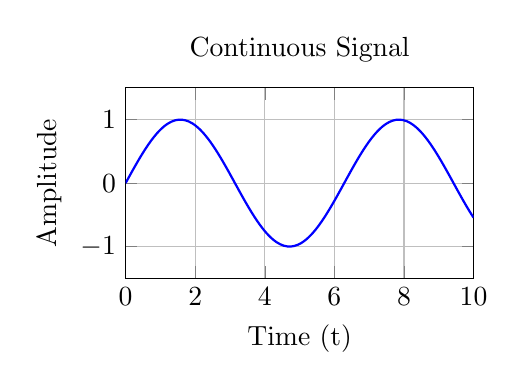
\begin{tikzpicture}
                \begin{axis}[
                    width=6cm, height=4cm,
                    xlabel={Time (t)},
                    ylabel={Amplitude},
                    title={Continuous Signal},
                    grid=major,
                    ymax=1.5, ymin=-1.5,
                    xmin=0, xmax=10
                ]
                    \addplot[domain=0:10, samples=100, smooth, thick, blue] {sin(deg(x))};
                \end{axis}
            \end{tikzpicture}

            \vspace{1cm} % Adding a gap between the two graphs

            % Sampled Signal Diagram
            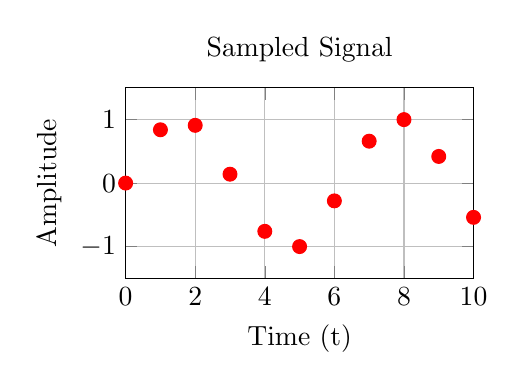
\begin{tikzpicture}
                \begin{axis}[
                    width=6cm, height=4cm,
                    xlabel={Time (t)},
                    ylabel={Amplitude},
                    title={Sampled Signal},
                    grid=major,
                    ymax=1.5, ymin=-1.5,
                    xmin=0, xmax=10
                ]
                    \addplot[only marks, mark=*, red, mark size=2.5pt] coordinates {
                        (0,0) (1,0.84) (2,0.91) (3,0.14) (4,-0.76) (5,-1) (6,-0.28) (7,0.66) (8,1) (9,0.42) (10,-0.54)
                    };
                \end{axis}
            \end{tikzpicture}
        \end{multicols}
    \end{center}

    \subsection*{\textbf{Explanation}}

    The first diagram represents the original continuous signal, which varies smoothly over time. This signal is then sampled, capturing discrete points at regular intervals. The second diagram shows the resulting sampled discrete points.


    




\[
s(t) \leftrightarrow s(\omega)
\]
\[
s(t) = m(t) \cdot c(t)
\]
\[
s(\omega) = \frac{1}{2\pi} \left[ M(\omega) * C(\omega) \right]
\]
\[
C(\omega) = \omega_s \sum_{n=-\infty}^{\infty} \delta(\omega - n\omega_s)
\]
\[
\Rightarrow s(\omega) = \frac{1}{2\pi} \left[ M(\omega) * \sum_{n=-\infty}^{\infty} \delta(\omega - n\omega_s) \right]
\]
\[
s(\omega) = \frac{1}{T_s} \sum_{n=-\infty}^{\infty} M(\omega - n\omega_s)
\]
\[
= \frac{1}{T_s} \left[ \sum_{n=-\infty}^{\infty} M(\omega - n\omega_s) \right]
\]
\[
= \frac{1}{T_s} \left[ \dots + M(\omega + \omega_s) + M(\omega) + M(\omega - \omega_s) + \dots \right]
\]

\begin{center}
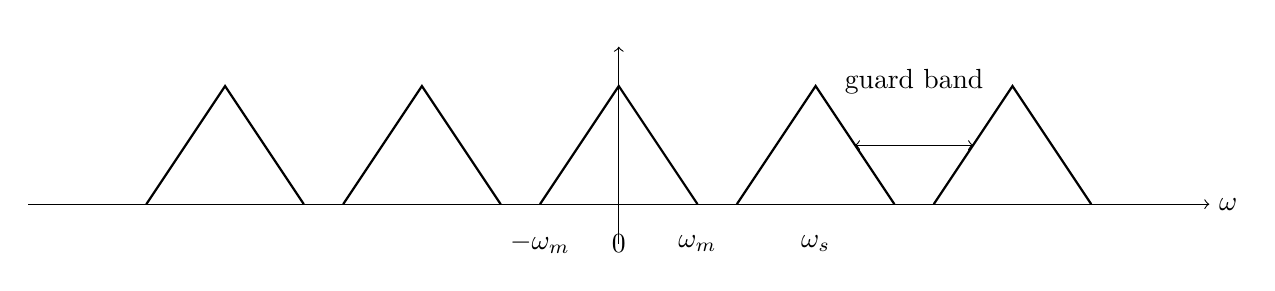
\begin{tikzpicture}
    % Draw x-axis and label
    \draw[->] (-7.5, 0) -- (7.5, 0) node[right] {$\omega$};
    % Draw y-axis
    \draw[->] (0, -0.5) -- (0, 2) node[above] {};
    % Draw triangles with slightly reduced spacing
    \foreach \x in {-5, -2.5, 0, 2.5, 5} {
        \draw[thick] (\x-1, 0) -- (\x, 1.5) -- (\x+1, 0);
    }
    % Label key points
    \node at (0, -0.5) {$0$};
    \node at (2.5, -0.5) {$\omega_s$};
   
    
    
    \node at (1, -0.5) {$\omega_m$};
    \node at (-1, -0.5) {$-\omega_m$};
    
    
    % Label guard band with updated position
    \draw[<->] (3, 0.75) -- (4.5, 0.75) node[midway, above, yshift=15pt] {guard band};
\end{tikzpicture}
\end{center}

\[
\Rightarrow \omega_s - \omega_m > \omega_m > \omega_s + \omega_m
\]
\[
\therefore \omega_s \geq 2\omega_m
\]

\section*{Recovery of Original Signal}
Recovery of the original signal is only possible when there is no overlapping.

\[
\omega_s > 2 \omega_m
\]

\begin{center}
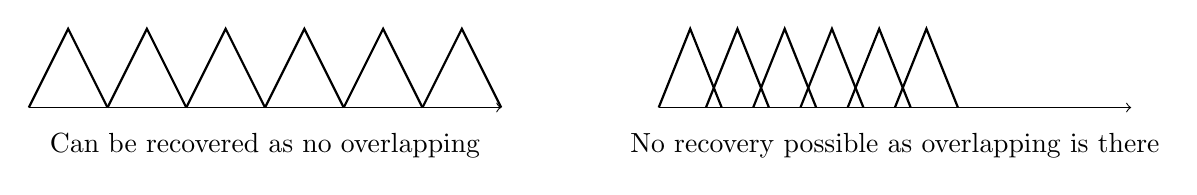
\begin{tikzpicture}
    % First graph - No overlapping
    \draw[->] (0,0) -- (6,0) node[right] {};
    \foreach \x in {0,1,2,3,4,5} {
        \draw[thick] (\x,0) -- (\x+0.5,1) -- (\x+1,0);
    }
    \node[below] at (3,-0.2) {Can be recovered as no overlapping};

    % Second graph - Overlapping
    \begin{scope}[xshift=8cm]
        \draw[->] (0,0) -- (6,0) node[right] {};
        \foreach \x in {0,0.6,1.2,1.8,2.4,3} {
            \draw[thick] (\x,0) -- (\x+0.4,1) -- (\x+0.8,0);
        }
        \node[below] at (3,-0.2) {No recovery possible as overlapping is there};
    \end{scope}
\end{tikzpicture}
\end{center}

\section*{Sampling Theorem}
A signal can be represented in its samples and can be recovered back when sampling frequency \( \omega_s \) is greater or equal to twice the maximum frequency component present in the signal \( (2 \omega_m) \).

\section*{Nyquist Rate \& Nyquist Interval}

\textbf{Oversampling:}
\[
\omega_s > 2 \omega_m \quad \Rightarrow \quad f_s > 2 f_m
\]

\textbf{Undersampling:}
\[
\omega_s < 2 \omega_m \quad \Rightarrow \quad f_s < 2 f_m
\]

\begin{center}
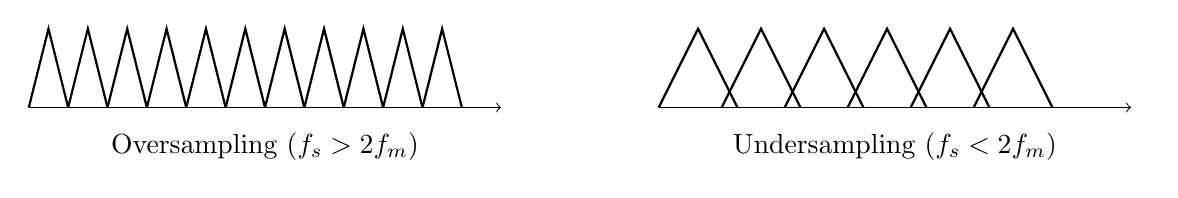
\begin{tikzpicture}
    % Oversampling graph
    \draw[->] (0,0) -- (6,0) node[right] {};
    \foreach \x in {0,0.5,1,1.5,2,2.5,3,3.5,4,4.5,5} {
        \draw[thick] (\x,0) -- (\x+0.25,1) -- (\x+0.5,0);
    }
    \node[below] at (3,-0.2) {Oversampling (\(f_s > 2 f_m\))};

    % Undersampling graph
    \begin{scope}[xshift=8cm]
        \draw[->] (0,0) -- (6,0) node[right] {};
        \foreach \x in {0,0.8,1.6,2.4,3.2,4} {
            \draw[thick] (\x,0) -- (\x+0.5,1) -- (\x+1,0);
        }
        \node[below] at (3,-0.2) {Undersampling (\(f_s < 2 f_m\))};
    \end{scope}
\end{tikzpicture}
\end{center}

When \( f_s = 2 f_m \), this is known as the \textbf{Nyquist Rate}.

\[
T_s = \frac{1}{2 f_m}
\]
Que: Find Nyquist rate and Nyquist interval for the following:
\[
m(t) = \cos 100 \pi t + 2 \sin 200 \pi t
\]

Sol.
\[
m(t) = x_1(t) + x_2(t)
\]
\[
x_1(t) = \cos 100 \pi t \Rightarrow \omega_1 = 100 \pi
\]
\[
x_2(t) = 2 \sin 200 \pi t \Rightarrow \omega_2 = 200 \pi
\]

\[
\omega_1 < \omega_2
\]

As we are looking for maximum frequency component:
\[
\omega_m = \omega_2 = 200 \pi
\]

\[
f_m = \frac{\omega_m}{2 \pi} = 100 \, \text{Hz}
\]

\[
\text{Nyquist rate} = 2f_m = 200 \, \text{Hz}
\]
\[
\text{Nyquist interval} \Rightarrow T_s = \frac{1}{f_s} = \frac{1}{200} = 5 \, \text{ms}
\]

\section*{Properties of Nyquist Rate}
\begin{enumerate}
    \item For a signal \( m(t) \) having Nyquist rate \( f_s \), \( m(t \pm t_s) \) has the same Nyquist rate, so the Nyquist rate does not change.
    
    \item For a signal \( m(t) \) having Nyquist rate \( f_s \), \( m(at) \) has Nyquist rate \( af_s \), which is known as \textit{time scaling}.
\end{enumerate}

\setlength{\parindent}{}
\setlength{\parskip}{0.5\baselineskip}
3. \quad ��m(t) \longrightarrow f(s)�� \\
\[
[m(t)]^n \longrightarrow n \times f(s) \quad
\begin{cases}
x(t) \longrightarrow \omega s, \\
(x(t))^2 \longrightarrow 2 \omega s
\end{cases}
\]
\vskip .2in
4. \quad ��m(t) \longrightarrow f(s)�� \\
\[
\frac{dm(t)}{dt} \longrightarrow f(s)
\]
\vskip .2in
5. \quad ��m(t) \longrightarrow f(s)�� \\
\[
\int_{-\infty}^{t} m(t) dt \longrightarrow \frac{f(s)}{s}
\]
\vskip .2in
6. \quad ��m_{1}(t) \longrightarrow f_{1}(s), \quad m_{2}(t) \longrightarrow f_{2}(s)�� \\
\[
m(t) = m_{1}(t) \cdot m_{2}(t) \longrightarrow f(s) = f_{s1} + f_{s2}
\]
\vskip .2in
\textbf{Question: Calculate Nyquist rate in rad/sec and in Hz}
\vskip .2in
\textbf{Solution:}
\[
m(t) = 2 \sin(4\pi t) \cos(2\pi t)
\]
Using trigonometric identities:
\[
m(t) = \sin(6\pi t) + \sin(2\pi t)
\]
Thus, the angular frequencies are:
\[
\omega_1 = 6\pi, \quad \omega_2 = 2\pi
\]
Therfore, maximum angular frequency iis, ��\omega_m = 6\pi��

Nyquist rate:
N.R
\[
\omega_nr= 2\omega_m = 12\pi \text{ rad/sec}
\]
\[
f_s = \frac{12\pi}{2\pi} = 6 \text{ Hz (Nyquist rate)}
\]
\section*{Question 1}
\textbf{Find the Nyquist rate for the following:}
\begin{enumerate}
    \item Sa$(4\pi t)$
    \item Sa$^3(5\pi t)$
    \item Sa$^2(4\pi t)$Sa$^4(5\pi t)$
\end{enumerate}

\section*{Solution}

\subsection*{1. Sa$(4\pi t)$}
The function Sa$(x)$, or sinc$(x) = \frac{\sin(x)}{x}$, is a low-pass signal with bandwidth determined by the highest frequency present in the argument of the sine function.

For Sa$(4\pi t)$, the argument of the sine is $4\pi t$. The highest frequency is determined from the term $4\pi$, which corresponds to a frequency of $2$ Hz (because $4\pi$ is $2 \times 2\pi$).

Therefore, the Nyquist rate is twice the highest frequency:

\[
f_N = 2 \times 2 \text{ Hz} = 4 \text{ Hz}.
\]

\subsection*{2. Sa$^3(5\pi t)$}
For Sa$^3(5\pi t)$, the argument of the sine is $5\pi t$. The highest frequency here is $\frac{5\pi}{2\pi} = 2.5$ Hz.

Thus, the Nyquist rate is:

\[
f_N = 2 \times 2.5 \text{ Hz} = 5 \text{ Hz}.
\]

\subsection*{3. Sa$^2(4\pi t)$Sa$^4(5\pi t)$}
In this case, we have a product of two sinc functions: Sa$^2(4\pi t)$ and Sa$^4(5\pi t)$. 

- For Sa$^2(4\pi t)$, the highest frequency is 2 Hz (as calculated previously).
- For Sa$^4(5\pi t)$, the highest frequency is 2.5 Hz (as calculated previously).

The overall signal will have the higher of these two frequencies dominating the bandwidth. Hence, the highest frequency is 2.5 Hz.

Thus, the Nyquist rate is:

\[
f_N = 2 \times 2.5 \text{ Hz} = 5 \text{ Hz}.
\]


\title{\Huge \textbf{Reconstruction of Signal}} 
\date{} % Leave date empty to omit it
\maketitle


\section*{Reconstruction of Signal}

\begin{center}
    \begin{tikzpicture}
       % Diagram of signal reconstruction
\node at (-6, 0) {$m(t)$};
\node at (-4, 0) {Sampler};
\node at (-2, 0) {$s(t)$};
\node at (0, 0) {LPF};
\node at (4.5, 0) {$m_r(t)$ (recovered message signal)};

% Arrows between blocks
\draw[->] (-5.5, 0) -- (-4.8, 0);
\draw[->] (-3.2, 0) -- (-2.5, 0);
\draw[->] (-1.5, 0) -- (-0.5, 0);
\draw[->] (0.5, 0) -- (1.3, 0);

% Arrow pointing to sampling frequency with further adjusted label placement
\draw[->] (-4, -0.5) -- (-4, -1.5);
\node[below] at (-4, -1.8) {$c(t), \omega_s$};


    \end{tikzpicture}
\end{center}

\[
H(\omega) = \frac{M_r(\omega)}{S(\omega)}
\]


\begin{center}
    % M(ω) graph
    \begin{tikzpicture}
        \draw[->] (-3,0) -- (3,0) node[right] {$\omega$};
        \draw[->] (0,-0.5) -- (0,2) node[above] {$M(\omega)$};
        \draw[-] (-1.5,0) -- (0,1.5) -- (1.5,0);
        \node[below] at (-1.5,0) {$-\omega_m$};
        \node[below] at (1.5,0) {$\omega_m$};
    \end{tikzpicture}

\end{center}


\[
\text{So } M_r(\omega) = H(\omega) \cdot S(\omega)
\]

\begin{center}
    % H(ω) graph
    \begin{tikzpicture}
        \draw[->] (-3,0) -- (3,0) node[right] {$\omega$};
        \draw[->] (0,-0.5) -- (0,2) node[above] {$H(\omega)$};
        \draw[-] (-2,1) -- (2,1);
        \draw[dashed] (-2,1) -- (-2,0) node[below] {$-\omega_c$};
        \draw[dashed] (2,1) -- (2,0) node[below] {$\omega_c$};
    \end{tikzpicture}

    \[
        \omega_c = \text{cutoff frequency}
    \]
\end{center}

\begin{center}
    % S(ω) graph
    \begin{tikzpicture}
        \draw[->] (-5,0) -- (5,0) node[right] {$\omega$};
        \draw[->] (0,-0.5) -- (0,2) node[above] {$S(\omega)$};
        \draw[-] (-4.0,0) -- (-3.0,1.5) -- (-2.0,0);
        \draw[-] (-1.0,0) -- (0,1.5) -- (1.0,0);
        \draw[-] (2,0) -- (3,1.5) -- (4,0);
        
        \node[below] at (1.0,0) {$\omega_m$};
        \node[below] at (3,0) {$\omega_s$};
    \end{tikzpicture}
\end{center}

\[
\text{So } M_r(\omega)
\]

\[
\omega_m \leq \omega_c \leq \omega_s - \omega_m
\]

As $\omega_c > \omega_m$, so we recover our signal. \\
At $\omega_c = \omega_m$, we recover our signal. \\
For $\omega_c < \omega_m$, 

\begin{center}
    % Clipped Fourier Transform graph
    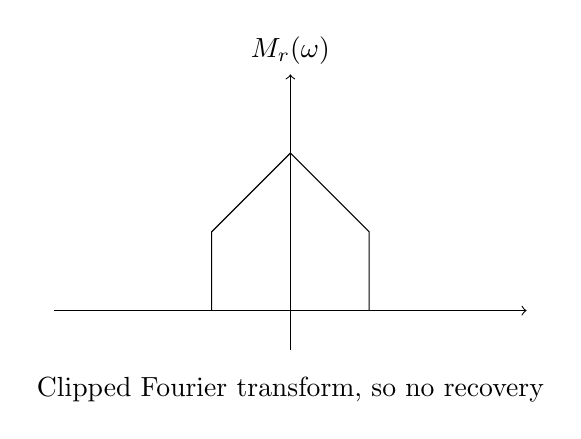
\begin{tikzpicture}
        \draw[->] (-3,0) -- (3,0) node[right] {};
        \draw[->] (0,-0.5) -- (0,3) node[above] {$M_r(\omega)$};
        \draw[-] (-1.,0) -- (-1.,1.) -- (0,2.0) -- (1.,1.) -- (1.,0);
        \node[below] at (-0.75,0) {};
        \node[below] at (0.75,0) {};
        \node[below] at (0,0) {};
        \node at (0,-1) {Clipped Fourier transform, so no recovery};
    \end{tikzpicture}
\end{center}

For overlapping signals:

\begin{center}
    \begin{tikzpicture}
        % Overlapping signal plot
        \draw[->] (-4,0) -- (4,0) node[right] {};
        \draw[->] (0,-1) -- (0,1.5) node[above] {};
        \draw[-] (-2.8,0) -- (-1.8,1) -- (-0.8,0);
        \draw[-] (-1,0) -- (0,1) -- (1,0);
        \draw[-] (0.8,0) -- (1.8,1) -- (2.8,0);
        \draw[-] (-1,0) -- (-1,1) -- (1,1) -- (1,0);
        
        
    \end{tikzpicture}
\end{center}

Fourier transform has extra parts so the original signal is not same to Fourier transform.

\newpage

\title{\textbf{\Huge Applications and Philosophical Insights of Sampling Theory}}
\date{}



\maketitle

\section*{\underline{\textbf{Applications of Sampling Theory}}}

Sampling theory has a wide range of practical applications across various fields due to its ability to simplify the analysis, processing, and interpretation of data. Here are some notable applications:

\subsection*{1. Digital Signal Processing (DSP)}
\begin{itemize}
    \item \textbf{Audio and Speech Processing:} Sampling enables the digitization of sound signals for applications like music streaming, voice recognition, and digital assistants. CDs, MP3s, and digital radio use sampled audio for playback and transmission.
    \item \textbf{Image Processing:} Sampling is essential in converting images from continuous analog signals to digital pixels, making it possible to process, store, and transmit images. Formats like JPEG and PNG rely on sampling for compression and storage.
    \item \textbf{Video Processing:} Video data is sampled to create frames that can be transmitted, stored, and edited. Formats like MP4 and streaming services like Netflix and YouTube rely on sampled video for efficient delivery.
\end{itemize}

\subsection*{2. Telecommunications and Data Transmission}
\begin{itemize}
    \item \textbf{Cellular Networks:} Voice signals in mobile communication are sampled and digitized for transmission over digital networks, allowing for better signal quality, encryption, and compression.
    \item \textbf{Internet Communication:} Voice-over-IP (VoIP) applications like Skype and Zoom convert analog voice signals into digital data using sampling, enabling clear, efficient communication over the internet.
    \item \textbf{Digital TV and Radio:} Television and radio stations sample audio and video signals for broadcast in digital form, which reduces bandwidth requirements and improves signal quality.
\end{itemize}

\subsection*{3. Medical and Biological Signal Processing}
\begin{itemize}
    \item \textbf{Medical Imaging:} Sampling theory is used in CT scans, MRI, and ultrasound imaging. Medical devices sample signals from the body, convert them to digital form, and reconstruct images for diagnostic purposes.
    \item \textbf{Electrocardiograms (ECG) and Electroencephalograms (EEG):} Sampling is used in ECG and EEG machines to record electrical activity in the heart and brain, allowing doctors to diagnose and monitor health conditions.
    \item \textbf{Wearable Health Monitors:} Devices like fitness trackers and smartwatches sample heart rate, oxygen levels, and other biological signals to provide real-time health monitoring.
\end{itemize}

\noindent Sampling theory enables efficiency, accuracy, and practicality across these fields, making it possible to analyze and process large-scale data in ways that would be impractical or impossible otherwise.

\newpage

\section*{\underline{\textbf{Philosophical Insight into Sampling Theory}}}

The philosophical aspects of sampling theory challenge our understanding of reality, perception, and knowledge. At its core, the theory—particularly the Nyquist-Shannon Sampling Theorem—suggests that a continuous phenomenon can be accurately represented by a finite number of discrete samples, provided the sampling rate is sufficient.

This idea raises intriguing questions about whether reality itself could be fundamentally discrete or, at least, sufficiently captured in a simplified, digital form. It parallels cognitive science theories suggesting that human perception operates on snapshots, or samples, of the world rather than continuous input, with the brain “filling in” the gaps to create a cohesive experience.

Sampling theory implies that complete knowledge of a system isn’t necessary to understand it fully; only certain critical points, or frequencies, are needed to reconstruct the whole. This resonates with minimalist and structural perspectives in philosophy, where simplified representations can still embody the essence of complex phenomena.

Additionally, the observer’s choice of sampling rate reflects the influence of perspective on knowledge, emphasizing that our understanding of reality may depend on how we choose to observe and interpret it. In essence, sampling theory blurs the line between continuity and discreteness, suggesting that finite, structured information can point toward a potentially infinite, continuous reality, bridging digital and analog views of existence.






\end{document}
